%% This is a sample manuscript marked up using the
%% AASTeX v5.x LaTeX 2e macros.

%% The first piece of markup in an AASTeX v5.x document
%% is the \documentclass command. LaTeX will ignore
%% any data that comes before this command.

%% The command below calls the preprint style
%% which will produce a one-column, single-spaced document.
%% Examples of commands for other substyles follow. Use
%% whichever is most appropriate for your purposes.
%%

%\documentclass[11pt,preprint2]{aastex}
% manuscript produces a one-column, double-spaced document:
%\documentclass[manuscript]{aastex}
%% preprint2 produces a double-column, single-spaced document:

%\documentclass{emulateapj}
\documentclass[preprint]{aastex}

\usepackage{natbib}
\usepackage{amsmath}
\bibliographystyle{apj}
\usepackage{graphicx}

\newcommand{\mintext}{\text{min}}
\newcommand{\maxtext}{\text{max}}
\newcommand{\rad}{\text{rad}}
\newcommand{\IR}{\text{IR}}
\newcommand{\ir}{\text{IR}}
\newcommand{\therm}{\text{therm}}
\newcommand{\cosmo}{\text{cosmo}}
\newcommand{\fg}{\text{fg}}
\newcommand{\res}{\text{res}}
\newcommand{\shot}{\text{shot}}
\newcommand{\SNR}{\text{SNR}}


%% Sometimes a paper's abstract is too long to fit on the
%% title page in preprint2 mode. When that is the case,
%% use the longabstract style option.

%% \documentclass[preprint2,longabstract]{aastex}

%% If you want to create your own macros, you can do so
%% using \newcommand. Your macros should appear before
%% the \begin{document} command.
%%
%% If you are submitting to a journal that translates manuscripts
%% into SGML, you need to follow certain guidelines when preparing
%% your macros. See the AASTeX v5.x Author Guide
%% for information.

%% You can insert a short comment on the title page using the command below.

%\slugcomment{Not to appear in Nonlearned J., 45.}

%% If you wish, you may supply running head information, although
%% this information may be modified by the editorial offices.
%% The left head contains a list of authors,
%% usually a maximum of three (otherwise use et al.).  The right
%% head is a modified title of up to roughly 44 characters.
%% Running heads will not print in the manuscript style.

\shorttitle{Foreground and sensitivity analysis for 21cm/Infrared studies}
\shortauthors{Neben et al.}

%% This is the end of the preamble.  Indicate the beginning of the
%% paper itself with \begin{document}.



\begin{document}

\title{First limits Foreground and sensitivity analysis for 21cm/Infrared intensity mapping correlation from the Epoch of Reionization}

%% Use \author, \affil, and the \and command to format
%% author and affiliation information.
%% Note that \email has replaced the old \authoremail command
%% from AASTeX v4.0. You can use \email to mark an email address
%% anywhere in the paper, not just in the front matter.
%% As in the title, use \\ to force line breaks.

\author{Abraham R. Neben\altaffilmark{1},
Brian Stalder\altaffilmark{2},
John L. Tonry\altaffilmark{2},
Jacqueline N. Hewitt\altaffilmark{1}}

\affil{\altaffilmark{1}MIT Kavli Institute, Massachusetts Institute of Technology, Cambridge, MA, 02139 USA}
\affil{\altaffilmark{2}Institute for Astronomy, University of Hawaii, 2680 Woodlawn Drive, Honolulu HI 96822}

%% Notice that each of these authors has alternate affiliations, which
%% are identified by the \altaffilmark after each name.  Specify alternate
%% affiliation information with \altaffiltext, with one command per each
%% affiliation.

%% Mark off your abstract in the ``abstract'' environment. In the manuscript
%% style, abstract will output a Received/Accepted line after the
%% title and affiliation information. No date will appear since the author
%% does not have this information. The dates will be filled in by the
%% editorial office after submission.

\begin{abstract}
aoeu
\end{abstract}

\keywords{cosmology: observations --- dark ages, reionization, first stars --- infrared: diffuse background}

\section{Introduction}

Deep radio and infrared observations are nearing detection of the first stars and galaxies from the cosmic dawn. As such sources form, they are thought to blow out ionized bubbles, eventually merging and reionizing the universe \citep{FurlanettoReview,miguelreview,PritchardLoebReview}. First generation 21\,cm observatories such the Murchison Widefield Array (MWA) \citep{tingay13,mwascience} and the Precision Array for Probing the Epoch of Reionization (PAPER) \citep{parsons14,ali15,PoberPAPER64Heating,DannyMultiRedshift} are setting ever tighter limits on redshifted neutral hydrogen emission from the neutral regions between these bubbles, and the now-underway Hydrogen Epoch of Reionization Array (HERA) \citep{deboer16} is expected to detect and characterize the EOR power spectrum in the coming years. Ultimately, the Square Kilometer Array (SKA) will image the EOR over redshift, revealing the hydrogen reionization history of the universe in detail \citep{ska}. 

At the same time, deeper galaxy redshift surveys are beginning to constrain the reionizing sources themselves. Hubble deep field observations \citep{Bouwens2011,Illingworth2013,Dunlop2013} and cluster lensing surveys are finding tens of galaxies at $6<z<10$ down to UV magnitudes of $M_{AB}\sim-17$, and extremely wide surveys are underway aiming to find rare extremely bright ones ones \citep{Schmidt2014,Trenti2011,Bradley2012}. However, current models require the contribution of far fainter galaxies down to $M_{AB}\sim-13$ \citep{Robertson2013,Alvarez2012} in order to agree with optical depth measurements \citep{planck16} from the cosmic microwave background. Deeper observations with the James Webb Space Telescope (JWST) \citep{Gardner2006} and the Wide Field Infrared Space Telescope (WFIRST) \citep{Spergel2013} will be needed to probe this crucial faint population \citep{Atek2015}.

Infrared intensity mapping offers several advantages compared to surveys. Power spectrum analyses can be sensitive to an EOR component even if the signal-to-noise in individual pixels small, and instead of being limited to the brightst galaxies, intensity mapping is sensitive to the cumulative light from \textit{all} sources. Indeed,  ionizing and Lyman-alpha radiation from EOR galaxies at $z\sim6-8$ redshifts into the near infrared, motivating intensity mapping at micron-scale wavelengths. Working around foregrounds is challenging, though. While early studies suggested angular fluctuations in infrared intensity maps traced EOR galaxies \citep[e.g.,][]{kash1,kash2,kash3}, \citet{kash4} find that given current constraints on the EOR, this is unlikely. In fact, \citet{cooray12,zemcov14} argue that intrahalo light, consisting of tidally stripped stars dispersed throughout host halos, is the best explanation for the observed fluctuation excess over known galaxy populations. This implies that even after significant foreground masking, EOR foreground emission in wide field infrared surveys is of order $10^4$ times brighter than EOR emission at $\sim10'$ scales.

Given these bright foregrounds, cross correlation with 21\,cm maps may in fact be the \textit{only} way to extract the diffuse EOR component of the near infrared background. The synergy is clear: the galaxies sourcing reionization generate strong Ly-$\alpha$ emission, while the neutral regions between them glow at rest frame 21\,cm. On scales larger than typical ionized bubbles, bright spots in IR maps likely correspond to ionized regions, and thus, 21\,cm dark spots, and vice versa, sourcing an anticorrelation seen in EOR simulations by \citet{StarsAndReionization,silva12,mao14,heneka16}. 

A similar anticorrelation on large scales is found by \citet{lidz09,park14} in simulations of 21\,cm cross correlation with galaxy surveys, but conducting redshift surveys both wide and deep enough to cross correlate with 21\,cm maps is an  challenge due to the wildly different spatial scales probed by 21\,cm experiments and deep galaxy surveys. The Hubble Ultra Deep Field, for instance, could fit inside a single resolution element in an MWA map. It may be possible to cross-check the ionization environment of deep JWST sources by comparing the brightness temperature in the 21\,cm map \citep{beardsley15}, but even after order $\sim100$\,hour integrations such detections will be near JWST limiting sensitivities \citet{zackrisson11}.

In contrast, intensity allows similar science with shallower observations, though imperfect radio and infrared foreground subtraction will leak largely uncorrelated power into the cross correlation analysis which must be averaged out over large fields of view. Fortunately the planned Transiting Exoplanet Survey Satellite \citep{ricker14} and the proposed SPHEREx mission \citep{ScienceWithSpherex,SpherexWhitePaper} would collect all sky near infrared maps, and many ground-based near infrared surveys with few degree fields such as the Dark Energy Survey \citep{des16}, Pan-STARRS \citep{tonry12}, and the Asteroid Terrestrial-impact Last Alert System (ATLAS) \citep{tonry11} are coming online. In the low frequency radio, the MWA has performed a deep survey of 400 square degrees at high galactic latitude \citep{beardsley16}, and HERA will survey $\sim2000$ square degrees along a zenith strip \citep{dillonmapmaking}. 

With wide and deep IR and low frequency radio surveys happening now and on the horizon, we study in this paper the real world prospects of detecting the cross correlation of diffuse 21cm and Ly-alpha emission from the EOR. We begin in Section 1 with a cross correlation analysis of radio and near infrared catalogs, setting upper limits on the level of foreground correlation, the presence of which would mask the cosmological correlation in sufficiently deep images. We then assess the correlation of faint, unresolved emission through a prototype 21cm/IR correlation analysis between wide band MWA and ATLAS images over a 10 degree field of view. After foreground subtraction and masking, we estimate typical foreground residual levels, and synthesize these with noise predictions into a sensitivity analysis for a larger scale image cross correlation experiment. We also make sensitivity predictions for a cube cross correlation experiment, quantifying the required infrared spectral resolution and taking advantage of avoidance of radio foregrounds using the ``EOR window''.

NEED TO INCORPORATE THIS PARAGRAPH
In this section we characterize the 21\,cm and IR foregrounds relevant to cross correlation measurements. We begin with bright point source foregrounds, demonstrating that distance variation of the sources combined with their finite luminosity distribution may introduce slight foreground correlations which compete with the cosmological signal. We study how well point source power spectra can be minimized with subtraction and masking, and after using these techniques we set the first limits on the 21\,cm--Ly$\alpha$ cross spectrum at $z=7$ using data from the MWA and ATLAS. Lastly, we calculate the sensitivities of several fiducial experiments, illustrating what it will take to realize this measurement.

\section{Power spectrum and correlation conventions}
\label{sec:pspecconventions}

\subsection{Power spectrum definitions}

We define the 3D power spectrum $P(\vec{k})$ of the image cube $I(x,y,z)$ following \citet{ewallwice14} as 
\begin{equation}
	P(\vec{k}) = \frac{\langle|\tilde{I}(\vec{k})|^2\rangle}{V}
\end{equation}
where
\begin{equation}
	\tilde{I}(\vec{k})=dV\sum_{\vec{x}}I(\vec{x})e^{i\vec{k}\cdot\vec{x}}
\end{equation}
and $V$ is the survey volume, and $dV$ is the voxel size.

Similarly, over narrow fields of view, the angular power spectrum $C_\ell$ of a 2D (e.g, broad band) image $I(\vec{\theta})$ can be shown to be approximately
\begin{equation}
\label{eqn:Cldef0}
	C(\vec{\ell}) = \frac{\langle|\tilde{I}(\vec{\ell})|^2\rangle}{\Omega} 
\end{equation}
where
\begin{equation}
	\tilde{I}(\vec{\ell})=d\Omega\sum_{\vec{\theta}}I(\vec{\theta})e^{i\vec{\ell}\cdot\vec{\theta}}
\end{equation}
and $\Omega$ is the survey solid angle, and $d\Omega$ is the pixel size. Thus, we need only evaluate a fourier transform to estimate $C_\ell$ over a narrow field of view. Writing this out in detail, we find\footnote{IS IT REALLY RIGHT THAT ALL THESE PEOPLE WROTE IT UP WRONG? ARE THERE DIFFERENT NORMALIZATIONS OF C$\ell$ ? Note that the normalization of $d\theta^2/N^2$ has been misstated as $1/N^2$ by \citet{zemcov14} (Eqn. 3 of their supplement), $d\theta$ by \citet{cooray12} (Eqn. 1 of their supplement), and $N^2d\ell^2/(2\pi)^2$ by \citet{thacker15} (Eqn. B3). Using Eqn. \ref{eqn:elldef}, the last form can be shown equal $1/d\theta^2$.} 
\begin{equation}
\label{eqn:Cldef}
	C(\ell(a,b))=\left\langle\left|\sum_{m,n}I(m,n)\exp\left(-\frac{2\pi i}{N}  (am+bn)\right)\right|^2\right\rangle\frac{d\theta^2}{N^2}
\end{equation}
where $d\theta=d\theta_x=d\theta_y$ is the pixel size, $N\equiv N_x=N_y$ is number of pixels on a side of a square image, and $\ell=\sqrt{\ell_x^2+\ell_y^2}$, where 
\begin{eqnarray}
\ell_x&=&2\pi a/N d\theta \label{eqn:elldef}\\
\ell_y&=&2\pi b/Nd\theta \label{eqn:elldef2}
\end{eqnarray}

Note that $C_\ell$ has the units of $[I^2d\theta^2]$. We will generally work with the dimensionally more intuitive power spectrum $\Delta(\ell)$, given by
\begin{equation}
	\Delta(\ell)=\sqrt{\frac{\ell^2}{2\pi}C(\ell)}
\end{equation}
which has the same units as I because $\ell$ has units of 1/rad. 

The 3D power spectrum is often cylindrically binned to $(k_\perp,k_\parallel)$ space where $k_\perp^2\equiv k_x^2+k_y^2$ represents modes perpendicular to the line of sight, and $k_\parallel=k_z$ represents modes along the line of sight. We show in Appendix \ref{sec:pspecrelation}  that this cylindrically binned power spectrum is related to the angular power spectrum of a broad band image (over a narrow field of view) as
\begin{equation}
P(k_\perp,k_\parallel=0)=D_c^2 \Delta D_c C_{\ell(k_\perp)}	
\end{equation}
with $\ell=D_c k_\perp$, where $D_c$ is the comoving line of sight distance to the center of the cube, and $\Delta D_c$ is the comoving depth of the cube.

\subsection{Cross spectrum vs. coherence}

We extend the definition of the angular power spectrum given in Eqn. \ref{eqn:Cldef0} to the cross spectrum as
\begin{equation}
\label{eqn:Cldefcross}
	C_{A,B}(\vec{\ell}) = \frac{\langle \tilde{I}_A^*(\vec{\ell})\tilde{I}_B(\vec{\ell})\rangle}{\Omega}
\end{equation}
where $A$ and $B$ denote the 21\,cm and the IR fields. The cross spectrum is a quantity which ranges between $\pm(C_{A}(\vec{\ell})C_{B}(\vec{\ell}))^{1/2}$ depending on how correlated or anti-correlated the two fields are. 

The cross spectrum is thus often renormalized as  
\begin{equation}
\label{eqn:Cldefcross}
	c_{A,B}(\vec{\ell}) \equiv \frac{C_{A,B}(\vec{\ell}) }{\sqrt{C_A(\vec{\ell})  C_B(\vec{\ell}) }}
\end{equation}
where $c$ is known as the coherence. The coherence quantifies the fractional correlation of the two fields, and is insensitive to a simple rescaling of either one. However, large foreground residuals afflicting either field will substantially bias the coherence towards zero \citep{lidz09,furlanettolidz07}. 

\section{Observations and Imaging}
\subsection{21\,cm Observations}

The MWA is a low frequency radio interferometer in Western Australia consisting of 128 phased array tiles, each with $\sim30^\circ\times(150\text{\,MHz}/f)$ field of view and steerable in few degree increments with a delay line beamformer. We use MWA low frequency radio observations of a quiet field centered at (RA,Dec)=($0^\circ$,$-27^\circ$) J2000 recorded over 30.72\,MHz bandwidth around 186\,MHz, corresponding to $z=6.0-7.3$. We begin with the 32 hours of observations calibrated, foreground-subtracted, and imaged by \citet{beardsley16}. These 32 hours result from applying stringent quality control cuts to roughly 80 hours of observations recorded between August and November 2013, where spectrally narrow RFI is flagged using COTTER \citep{AndreMWARFI}, based on AOFlagger\footnote{http://aoflagger.sourceforge.net} \citep{aoflagger} and spectrally broad RFI is flagged by comparing the spectral smoothness of the data compared to baseline levels. 

The 32 hours of observations are processed separately by \citet{beardsley16} as in 2 minute snapshots, and imaging is conducted using Fast Holographic Deconvolution\footnote{https://github.com/EoRImaging/FHD} \citep{fhd}. Model visibilities are predicted from a foreground model of diffuse and point source emission in the field \citep{beardsley16,PattiCatalog1}, to be used for both calibration and foreground subtraction. For each snapshot, FHD produces naturally weighted data and model image cubes as well as primary and synthesized beam cubes. We flag the upper and lower 80\,kHz channels in each of 24 coarse channels across the band to mitigate aliasing, and average the remaining channels in frequency to make a broad band image. 

FHD outputs these ``cubes'' in HEALPix format per frequency. Note that this processing is performed in parallel on ``odd'' and ``even'' data cubes whose data are interleaved in time to allow more leverage on estimating the magnitude of the noise and the noise bias. We average the cubes in frequency, rotate them so the EOR0 field center lies at the north pole, and project the pixels into the $xy$ plane, resulting in an orthographic projection to the plane tangent to  $(\text{RA}, \text{Dec})=(0,-27^\circ)$.

21\,cm intensity mapping measurements in 3D are limited by radio thermal noise, and demand order thousand hour integrations to reveal the cosmological signal \citep{beardsley13,PoberNextGen}. However in broadband measurements, thermal noise is subdominant to foreground residuals. Further, we expect to require large fields of view to recover any cosmological correlation between broadband 21\,cm and IR images. To that end, we examine whether all 32 hours are needed to achieve the lowest foreground residuals, or whether a subset will suffice. In fact, the $uv$ plane is essentially full after only 3 hours of rotation synthesis, and compounding days together serves only to increase signal to noise. 

In Fig. \ref{fig:respspecspacingsstudy} we compare the power spectra of the deep 32 hour integration (black dashed) to those of 3 hour integrations spread over 1 (red), 14 (green), and 166 (blue) nights. Each consists of 100 two-minute integrations with a minimum spacing of 0, 5, and 24 minutes, all with occasional several day gaps due to observing constraints and quality cuts. We plot the \textit{raw} spectra, the \textit{residual} spectra after foreground model subtraction, as well as the spectra of the odd--even difference cube which quantify the level of thermal noise. All four sets have the same raw power spectra, but the residual power spectrum decreases as the 3 hours are spread over more and more nights until it reaches the level of the deep 32 hour integration. These findings are consistent with ionosphere-related errors, e.g., in interferometric calibration, whose temporal correlations require many independent nights to average down. Thus while we use the 32 hour integration for convenience in this analysis, it is by no means necessary to use such a deep integration in a broad band analysis, especially when we will find later that survey speed is essential for such broad band correlation experiments. Note that thermal noise is vastly subdominant to foreground residuals in this broadband power spectrum.

\begin{figure}[h]
\centering
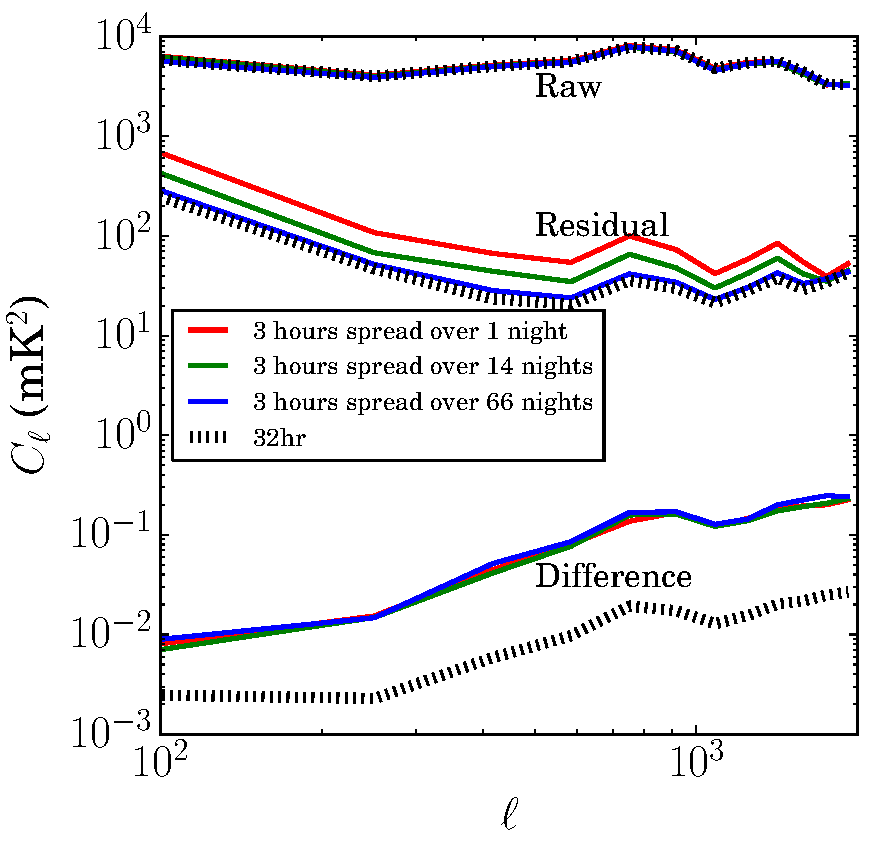
\includegraphics[width=4in]{images/res_pspec_of_100_obsids_with_diff_spacings.pdf}
\caption{CHANGE  ''DIFFERENCE'' TO THERMAL NOISE, CHANGE THE NUMBER OF DAYS TO BE THE NUMBER OF DIFFERENT NIGHTS OBSERVED, NOT SIMPLY THE END DAY MINUS THE FIRST DAY, WHICH INCLUDES WEEKENDS}
\label{fig:respspecspacingsstudy}
\end{figure}

\subsection{IR Observations}

\begin{figure}[h]
\centering
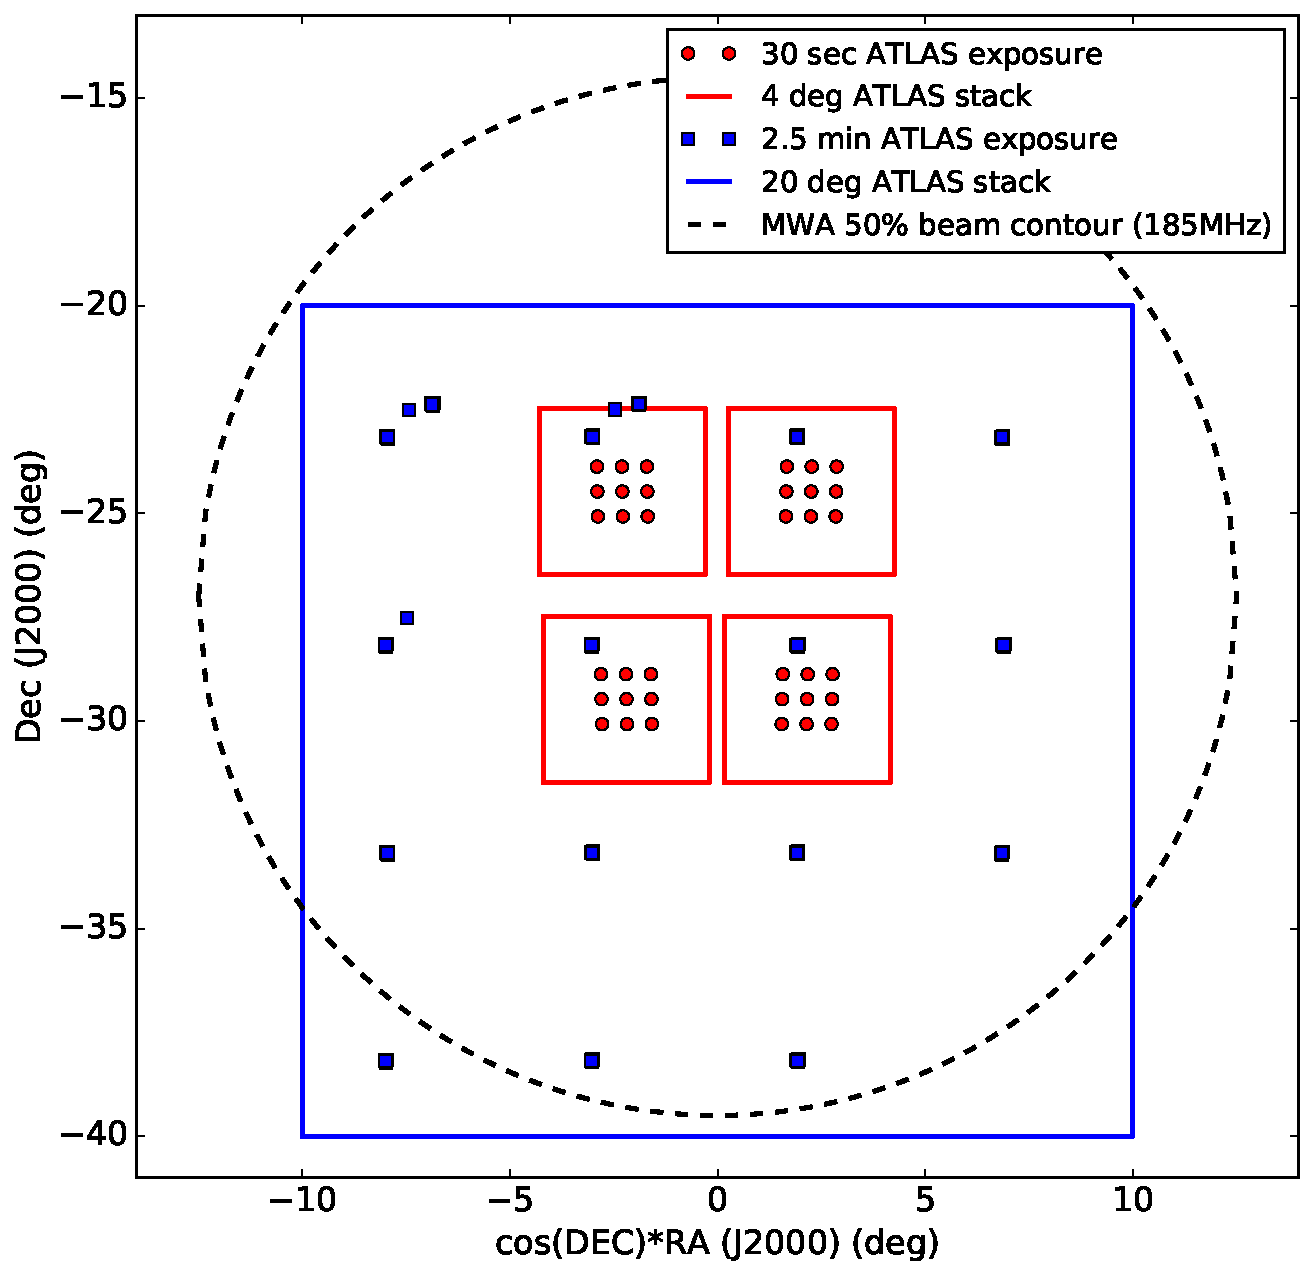
\includegraphics[width=4in]{images/survey_overview.pdf}
\caption{5' pixels}
\label{fig:surveyoverview}
\end{figure}

ATLAS is a 0.5\,m (f/2.0) telescope \citep{tonry11} in Hawaii designed to perform a wide field sky survey for near earth asteroids. The detector is a 10,500 $\times$10,500 STA-1600 CCD array, with a pixel scale of 1.86'', with an overall field of view of $5.5^\circ$. We observe in the I band centered at 807\,nm with full width at half max 150\,nm, corresponding to $z=$5.1--6.3. While this redshift range doesn't exactly match that of our r radio observations, it overlaps sufficiently for our purpose of characterizing the effects of noise foregrounds in 21cm--IR cross correlation experiments. 

We perform two separate observing campaigns, which we illustrate in Fig. \ref{surveyoverview}. We first perform a wide survey to best characterize bright foregrounds; . In the first campaign we raster scan a roughly $20^\circ\times20^\circ$ grid with $5^\circ$ spacing over the MWA field (dashed black circle), integrating for 2.5\,min at each pointing (blue square markers). The observations are conducted between 2016/09/07 22:00  and 2016/09/08 00:50 Hawaii-Aleutian Standard Time, when the moon was 36\% illuminated.  Later we will find that this is substantially more integration time than required to mitigate photon shot noise, but not enough to mitigate diffuse airglow structure and CCD array systematics. Still, it is sufficient for performing a source survey where source fluxes are estimated relative to the local background. 

We then use {\tt swarp}\footnote{http://www.astromatic.net/software/swarp} \citep{swarp} to stack all these frames over $20^\circ$ orthographic field centered on (RA,Dec) = $(0^\circ,-30^\circ)$ (blue square) with 1.86'' resolution. We use the default background subtraction settings to mitigate temporal and spatial background variation. 

% moon phase calculator: http://www.moonpage.com/index.html?go=T&auto_dst=T&tzone=ut&m=9&d=8&y=2016&hour=0&min=51&sec=45

Our second campaign is a deep survey designed to better mitigate airglow fluctuations and CCD systematics for the purpose of studying faint foregrounds. We select four 5 deg fields positioned around the MWA beam peak for best cross correlation precision: (RA,Dec) = $(-2.5^\circ, -24.5^\circ)$, $(2.5^\circ, -24.5^\circ)$, $(-2.5^\circ, -29.5^\circ)$, $(2.5^\circ, -29.5^\circ)$ (J2000). We raster scan a $3\times3$ grid of 30\,sec observations within each field (red circle markers) intended to mitigate slight amplifier non-uniformities across the CCD array. The observations were conducted on 2016/11/02 between 21:47 and 23:11 Hawaii-Aleutian Standard Time, when the moon was 5\% illuminated.

We stack the frames in each of the four deep fields using {\tt swarp}, saving only the central $4^\circ\times 4^\circ$ region over which all nine 30\,sec frames overlap (red squares). Otherwise slight background discontinuities would be introduced by the different temporal coverage of different regions of the stack. In this stacking, we disable background subtraction for the purpose of studying later on the effects of airglow-induced diffuse backgrounds.




\section{Point source foregrounds}

\subsection{Catalogs}

To characterize the bright sources relevant to 21\,cm--Ly$\alpha$ and  21\,cm--H$\alpha$ intensity mapping correlation measurements we calculate the correlations between catalogs at 185\,MHz, 850\,nm, and 4.5\,um as a function of mask depth. These bands correspond roughly to 21\,cm, Ly$\alpha$, and H$\alpha$ at $z\sim6-7$. 

\begin{figure*}[h]
\centering
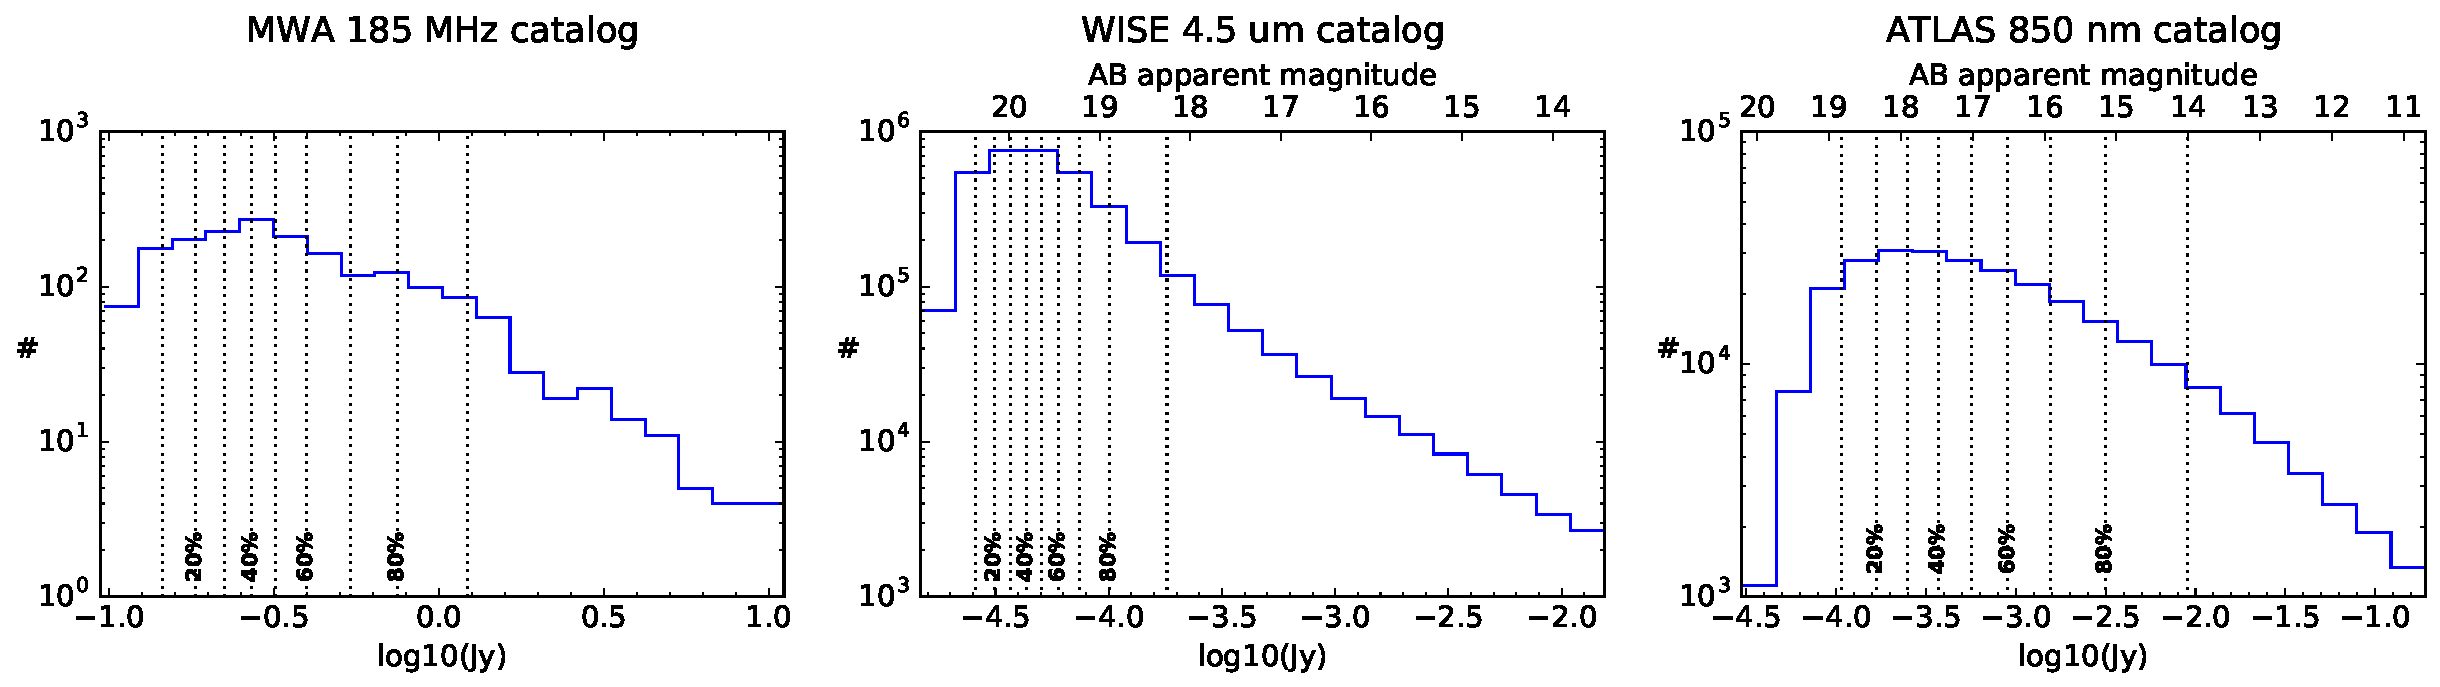
\includegraphics[width=6.5in]{images/catalog_histograms.pdf}
\caption{5' pixels}
\label{fig:cataloghistograms}
\end{figure*}

We use the 185\,MHz catalog reduced from deep observations of the MWA field depicted in Fig. \ref{fig:surveyoverview} by \citep{PattiCatalog1} (left panel in Fig. \ref{fig:cataloghistograms}). Unlike the other catalogs we consider, the survey depth varies somewhat over the MWA field due to the varying primary beam, though within the full-width-at-half-max it is complete to roughly 100\,mJy. MWA astrometry is at the 2--3' level due to the MWA's short baselines, though \citep{PattiCatalog1} cross-match MWA detections with higher frequency catalogs to achieve order 10'' astrometry. 

We use the W2 band of ALLWISE \citep{Wright2010,allwise} as our 4.5\,um catalog. We download the list of sources within the MWA field using the All Sky Search on the NASA/IPAC Infrared Science Archive\footnote{http://irsa.ipac.caltech.edu} (center panel in Fig. \ref{fig:cataloghistograms}). This ALLWISE band is specified to be 95\% complete to 88\,$\mu$Jy (15.7 AB mag), though it has slight sky coverage non-uniformities due to satellite coverage. We will see that we run into sky coverage problems only after masking the brightest 90\% of sources.

Lastly, we run SExtractor\footnote{http://www.astromatic.net/software/sextractors} \citep{sextractor} on our wide $20^\circ$ wide ATLAS composite image to generate an 850\,nm catalog. We allow local background bias and noise estimation, and set pixel saturation at 20,000 counts to avoid artifacts. We find the catalog is complete to roughly a mJy (right panel in Fig. \ref{fig:cataloghistograms}). 





flux-induced correlation calculations and maybe simulations of how flux cuts affect the correlations

\subsection{Point source correlations}

Having prepared catalogs of point source foregrounds in our three bands, we proceed to study how they manifest in intensity mapping correlation experiments. Traditionally, radio/optical/infrared correlations have been studied by cross matching high frequency radio detections with optical and infrared sources coincident within a few arcseconds, and plotting radio versus optical or infrared luminosity. Such studies have revealed the well known radio--far infrared correlation (CITATIONS) thought to be due to massive star formation \citep[e.g.][]{helou85,dejong85,yun01,xu94}. Such stars emit ionizing radiation which is reprocessed into far-infrared by dust, and also create HII regions which emit radio synchrotron \citep{xu94}. A secondary radio mechanism is synchrotron radiation from acceleration of cosmic ray electrons in these stars' supernovae. 

Our approach is different. For all the advantages of broad band intensity mapping, sources cannot be localized to specific redshifts, meaning that it is foreground fluxes, not luminosities, whose correlations are of interest. Of course compact foregrounds may be masked or subtracted to some residual level, but any correlation of these residual foreground fluxes could mask the cosmological correlation. We begin in this section by analyzing foreground fluxes as a function of masking depth, and in the next section turn to the foregrounds in residual images below the detection limit of these catalogs. A last comment on our approach is that though searching for radio--infrared correlations on a source-by-source level would be valuable cross check, we lack the radio astrometry to do so\footnote{In their cross matching study of GHz radio sources with optical detections, \citep{mcmahon02} find that 99\% of cross-matches within 10'' of each other (see their Fig. 8), of order the positional accuracy quoted by \citet{PattiCatalog1}.}. 

\begin{figure*}[h]
\centering
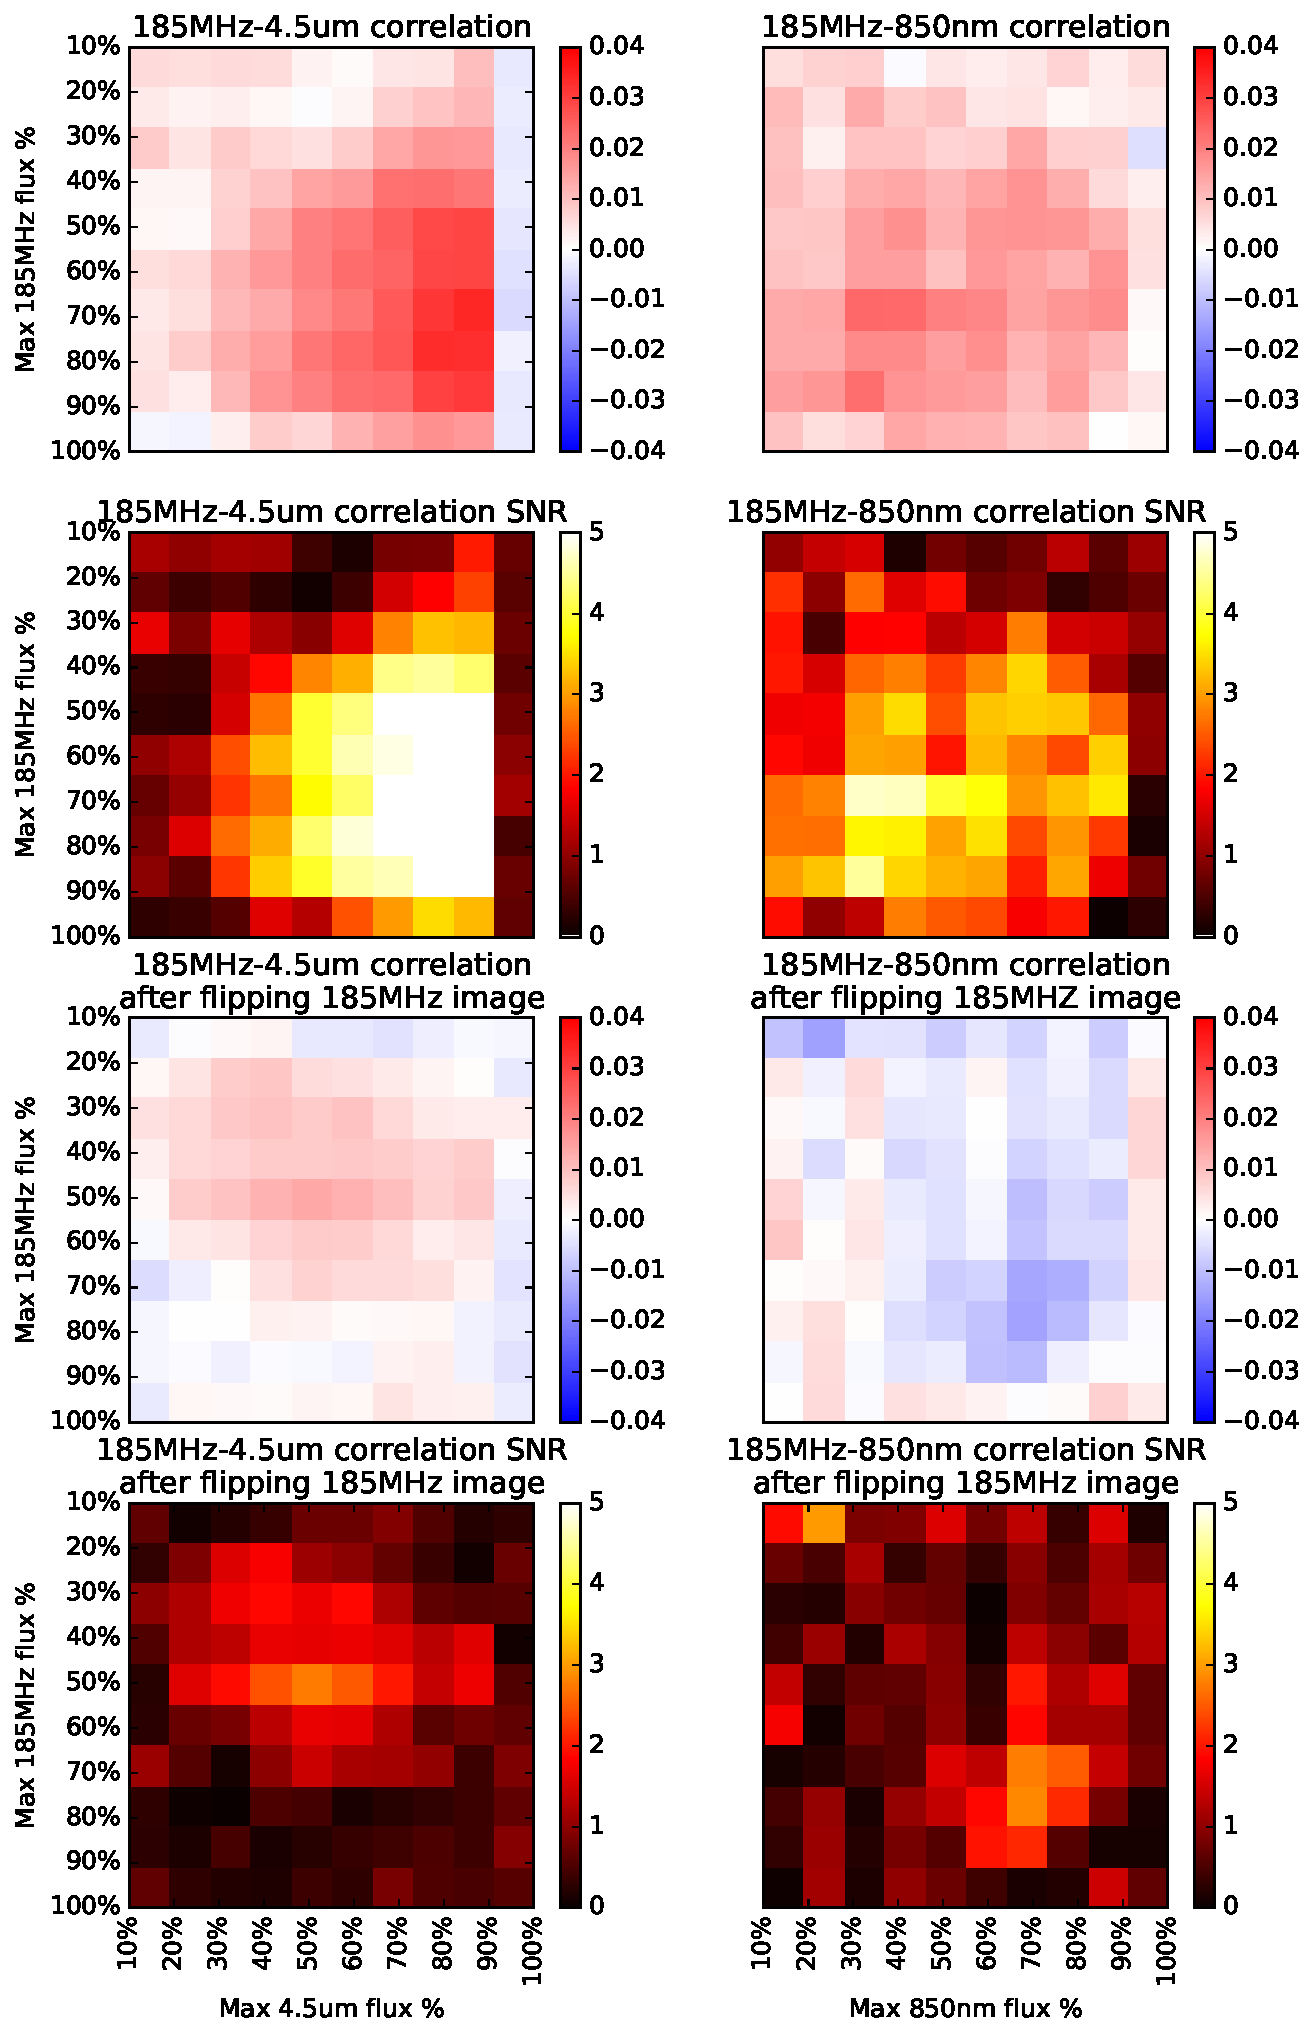
\includegraphics[width=5.5in]{images/source_correlation_grids_and_snrs.pdf}
\caption{5' pixels}
\label{fig:correlationsandSNRs}
\end{figure*}

We begin by gridding all three catalog fluxes in Jy to the $20^\circ\times20^\circ$ grid centered at (RA,Dec) = $(0, -30^\circ)$ depicted in Fig. \ref{fig:surveyoverview}, and calculating the zero delay correlations between the images $I_i(\theta_x,\theta_y)$ as
\begin{equation}
	c = \frac{\langle I_1I_2\rangle-\langle I_1\rangle\langle I_2\rangle}{\sqrt{(\langle I_1^2\rangle -\langle I_1\rangle^2)(\langle I_2^2\rangle -\langle I_2\rangle^2)}}
\end{equation}
where the sample variance in the case of small or zero correlation is dominated by the numerator and is given by $1/\sqrt{N_\text{pix}}$, where $N_\text{pix}$ is the total number of pixels in the image. Between MWA and WISE catalogs we find $c=-0.003\pm0.005$ and between MWA and ATLAS catalogs we find $c=0.0013\pm0.005$. Both are consistent with zero, which is not necessarily unexpected. The brightest sources in both infrared catalogs are likely stars, whose radio emission is vanishingly small. To illustrate, we calculate the correlations after excluding the brightest 10\% of sources in all three catalogs, and find $c_\text{MWA--WISE}=0.031\pm0.005$ and $c_\text{MWA--ATLAS}=0.0086\pm0.005$. The former is a $6\sigma$ detection, and merits some investigation. How does this apparent correlation depend on the flux cut? What is it due to? And what does it mean for broad band correlation experiments? Further, does the MWA--ATLAS correlation remain consistent with zero at stricter flux cuts?

To begin to answer these questions, we plot in Fig. \ref{fig:correlationsandSNRs} the 185\,MHz--4.5\,$\mu$m correlation (top left) and 185\,MHz--850\,nm correlation (top right) as a function of the maximum flux percentile not excluded from the data. For instance, the correlations we calculated above without any source masking are in the 100\%--100\% bin, while the correlation after removing the brightest 90\% of sources in both catalogs are in the 10\%--10\% bin. We indicate the fluxes that these percentiles correspond to in Fig. \ref{fig:cataloghistograms}. We plot the SNRs of these correlation measurements, taking the noise to be $1/\sqrt{N_\text{pix}}$ as described above, in the next row. Note that adjacent cells in the correlation matrix plots are strongly correlated, so a consistent positive sign is not in and of itself evidence of significance. We assess significance by comparing of each correlation measurement with the expected noise (the SNR), by checking that the correlation vanishes when the 185\,MHz image is flipped (bottom two rows).

The 185\,MHz and 4.5\,$\mu$m catalogs exhibit a positive correlation peaking at $0.0337\pm0.005$ after masking the brightest 10\% of 4.5\,$\mu$m sources (down to 18.25 mag) and the brightest 30\% of radio sources (down to 0.54\,Jy). The correlation is detected at greater than $3\sigma$ significance until either radio sources are masked down to the 0.2\,Jy level or 4.5\,$\mu$m sources are masked down to (19.8 mag) level. These levels are near the completeness limits of both catalogs, though, and even if the correlation extended to fainter fluxes is would not likely be significantly detected. There is no significant correlation detection after flipping the 185\,MHz image, indicating this is not an artifact of the analysis. The 185\,MHz and 850\,nm catalogs exhibit a smaller correlation, but one which nonetheless peaks at 3--4$\sigma$ significance over a broad range of flux cuts. This correlation peaks at $0.023\pm0.005$ after masking the brightest 30\% of 185\,MHz sources (down to 0.2\,Jy) and the brightest 70\% of 850\,nm sources (down to 17.9 mag). As before, this correlation vanishes as expected when the 185\,MHz image is flipped prior to cross correlation.

To understand these findings, we begin by digging deeper into the 4.5\,$\mu$m catalog. We select the subset of sources detected in WISE 3.4\,$\mu$m, 4.5\,$\mu$m, and 12\,$\mu$m bands and plot them (Fig. \ref{fig:wisecolorcolor}, left panel) in the $W_{23}\equiv$[4.6\,$\mu$m] -- [12\,$\mu$m] versus $W_{12}\equiv$[3.4\,$\mu$m] -- [4.6\,$\mu$m] color-color space used by \citet{Wright2010} to illustrate the separation of stars and various types of non-active and active galaxies. \citet{nikutta14} study how these different sources separate more quantitatively, finding that stars separate clearly from all other sources in the region $W{12}=-0.04\pm0.03$, $W_{23}=0.05\pm0.04$ (1$\sigma$). In the right panel, we plot the faintest 90\% of sources (fainter than 18.25 mags at 4.6\,$\mu$m) in the same color-color space and observe that all stars are excluded. This explains why before masking this brightest 10\%, we observed zero correlation with 185\,MHz sources, and why afterward the correlation suddenly emerges, after all, nearly all radio sources are non-stellar (i.e., extragalactic). 

\begin{figure}[h]
\centering
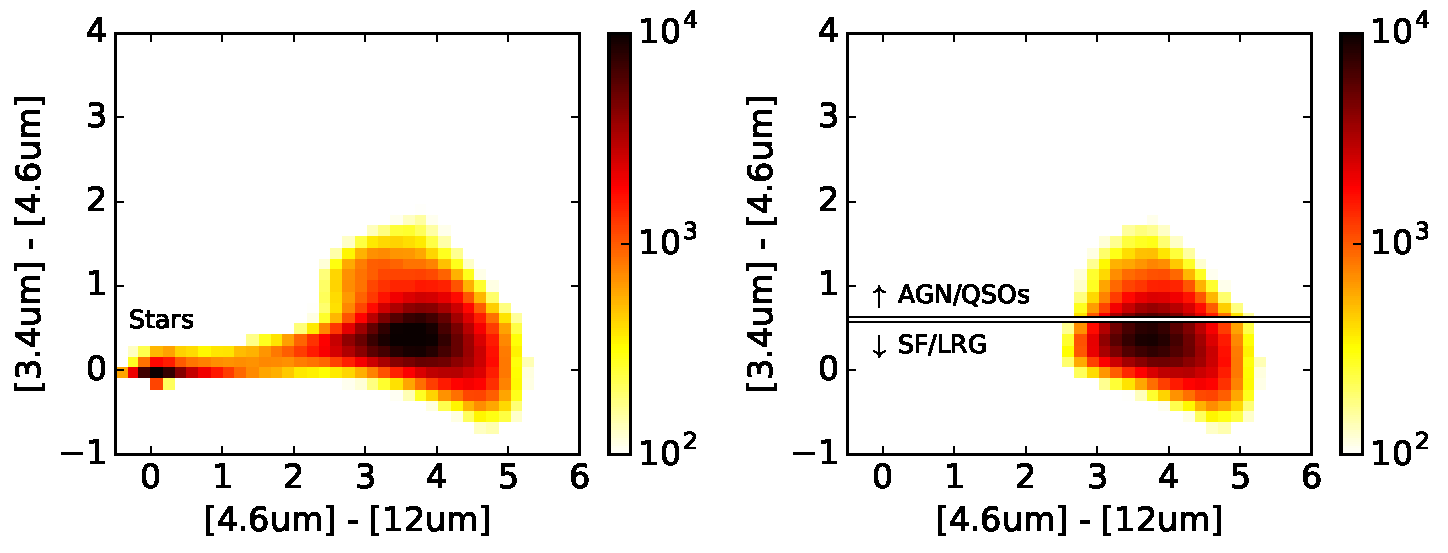
\includegraphics[width=6in]{images/wise_color_color_figure.pdf}
\caption{5' pixels}
\label{fig:wisecolorcolor}
\end{figure}

To further probe which infrared sources are responsible for this correlation, we make a simple cut to separate quasars (QSOs) and active galactic nuclei (AGNs) ($W_{12}>0.16$) from luminous red galaxies (LRGs) and starburst galaxies (SFs) ($W_{12}<0.16$) \citep{nikutta14,kurcz16}. In Fig. \ref{fig:wisexspec} we plot the power spectrum of 185\,MHz sources (left panel), the spectra of our QSO/AGN and LRG/SF cuts of 4.5\,$\mu$m sources (center panel), and the coherence (i.e., correlation coefficient versus $\ell$) of each of these cuts with the 185\,MHz catalog (right panel). The QSO/AGN subset exhibits no significant correlation with the 185\,MHz sources, while the LRG/SF cut exhibits a significant correlation rising from a few percent at $\ell\sim7000$ to 13\% at $\ell\sim300$. The falloff towards high $\ell$ is due to the 2' resolution of the MWA synthesized beam at 185\,MHz, corresponding to a maximum $\ell$ of roughly 6000. 

\begin{figure}[h]
\centering
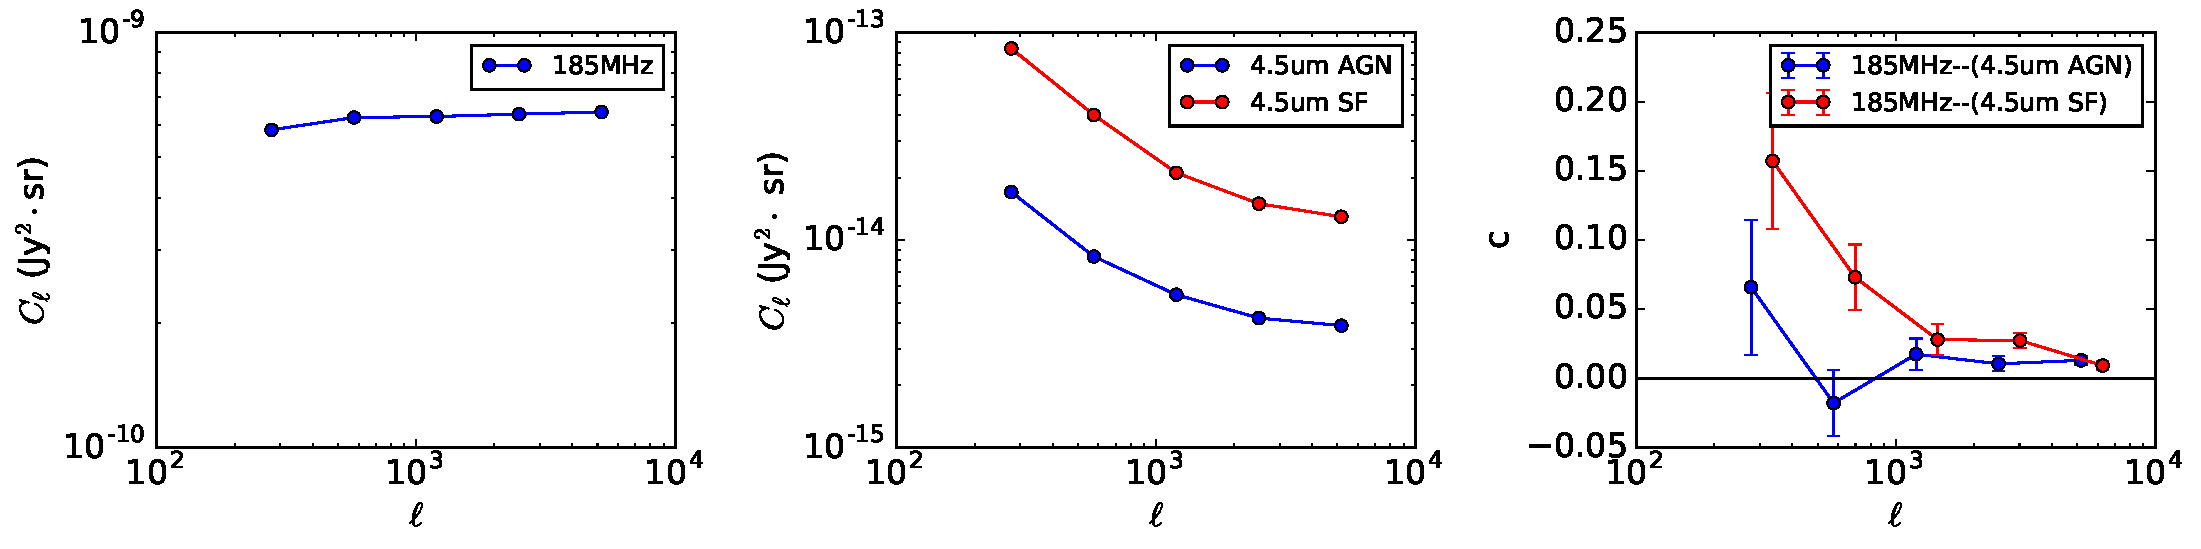
\includegraphics[width=7in]{images/mwa_wise_qsoagn_gal_xspec.pdf}
\caption{5' pixels}
\label{fig:wisexspec}
\end{figure}

%argue that LRGs are negligible in terms of radio emission compared to LRGs

The fall of the correlation towards high $\ell$ is due to the similar fall in the 4.5\,$\mu$m catalog power spectrum towards high $\ell$. Both the falling 4.5\,$\mu$m catalog power spectrum and the relatively  which are complex functions of the survey properties. \citet{tegmark02,dodelson02} show that the galaxy angular power spectrum $C_\ell$ is approximately equal to the 3D matter power spectrum $P(k(\ell))$ convolved with with a window function which depends on the redshift coverage and flux limit of the sample. The matter power spectrum is known to rise as $k^{1}$ for $k\lesssim0.02$\,h/Mpc, above which it falls as $k^{-3}$. Galaxy surveys typically probe the regime just above the turnover where the slope is transitioning from 0 to -3 \citep{tegmark02b}. In order to maximize its sensitivity to low surface EOR 21\,cm emission, the MWA was designed as a relatively compact array in comparison to higher resolution radio interferometers such as the Very Large Array. This low resolution makes the MWA catalog severely flux limited \citep{PattiCatalog1}, which in turn effectively masks many galaxies which would otherwise be seen. This large spatial mask translates into a wide fourier convolution kernel, explaining why the MWA catalog power spectrum is so flat.

Let us now turn to addressing why the 4.5\,$\mu$mu LRG/SF sample is 5--15\% correlated with the 185\,MHz catalog, while the QSO/AGN sample is not. Of course some slight correlation is expected at some level as brighter AGN are typically in more massive galaxies, which are typically brighter in stars as well (see, for instance, Fig. 1 in \citep{seymour07} or Fig. 4 in \citep{Willott03}) however \citet{mauch07} find no evidence of a radio/near-infrared luminosity correlation anywhere near as strong as that between radio and far-infrared emission. 

As discussed above, broadband intensity mapping is concerned not with a luminosity correlation, but with a flux correlation, and we thus attempt quantify to what extent fluxes in two different bands may appear correlated due to distance effects even when their intrinsic luminosities are completely independent of each other. By distance effects we refer to to the effect that more distant objects are generally weaker in all bands than nearer objects, and broadband intensity mapping is unable to remove this induced correlation.

INTRODUCE MY LUMINOSITY--FLUX ANALYTIC CALCULATION, AND DO IT USING THE RADIO AND IR LUMINOSITY FUNCTIONS IN THE "good luminosity functs" mendeley folder

\citet{mauch07}
\citet{fu10}


\begin{figure}[h]
\centering
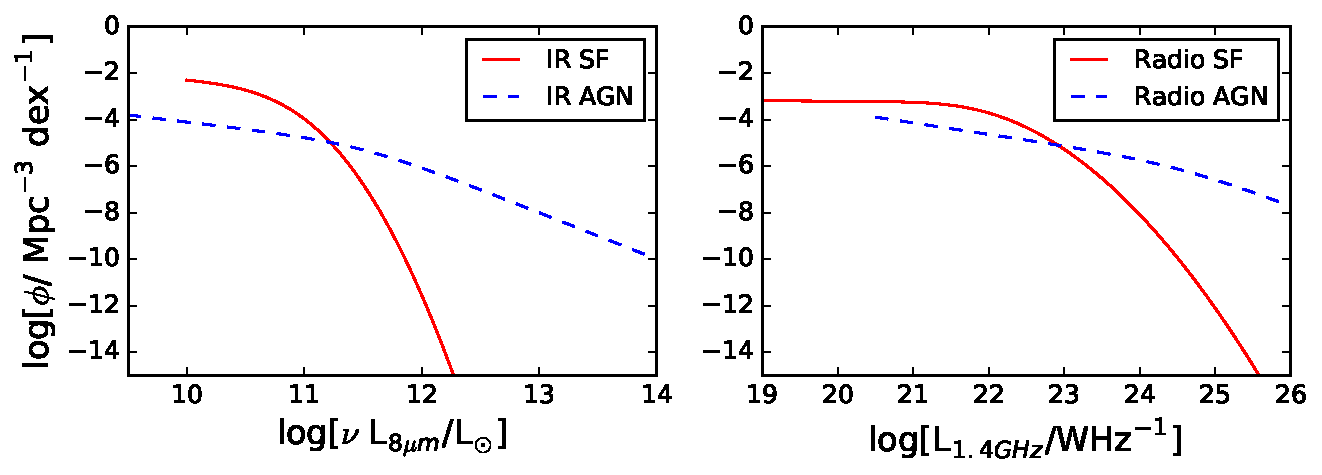
\includegraphics[width=6in]{images/sim_rad_ir_luminosity_functions.pdf}
\caption{5' pixels}
\label{fig:luminosityfunctions}
\end{figure}
talk about matching the number densities by fiddling with the minimum luminosities, and say a few words about how it doesn't really matter

% https://www.evernote.com/shard/s316/nl/2147483647/8270de10-6438-4d98-847a-a13e40ff9a14/
\begin{equation}
	c = \frac{\langle F_\rad F_\ir \rangle-\langle F_\rad\rangle\langle F_\ir\rangle}{\sqrt{(\langle F_\rad^2\rangle-\langle F_\rad\rangle^2)(\langle F_\ir^2\rangle-\langle F_\ir\rangle^2)}}
\end{equation}
Using $F_i=L_i/4\pi d^2$ for $i=\rad,\ir$, we find
\begin{equation}
	c = \frac{\beta-1}{\sqrt{(\beta\alpha_\rad-1)(\beta\alpha_\ir-1)}}
\end{equation}
where $\beta\equiv\langle d^{-4}\rangle/\langle d^{-2}\rangle^2$ and $\alpha_i=\langle L_i^2\rangle/\langle L_i\rangle^2$.
do this per source instead of per-pixel. For a survey of a fixed angular field of view, the distribution of source distances $d$ grows as $d^2$, and 
\begin{equation}
	\beta\approx\frac{d_\maxtext^3-d_\mintext^3}{3d_\maxtext d_\mintext (d_\maxtext-d_\mintext)}
\end{equation}





\begin{figure}[h]
\centering
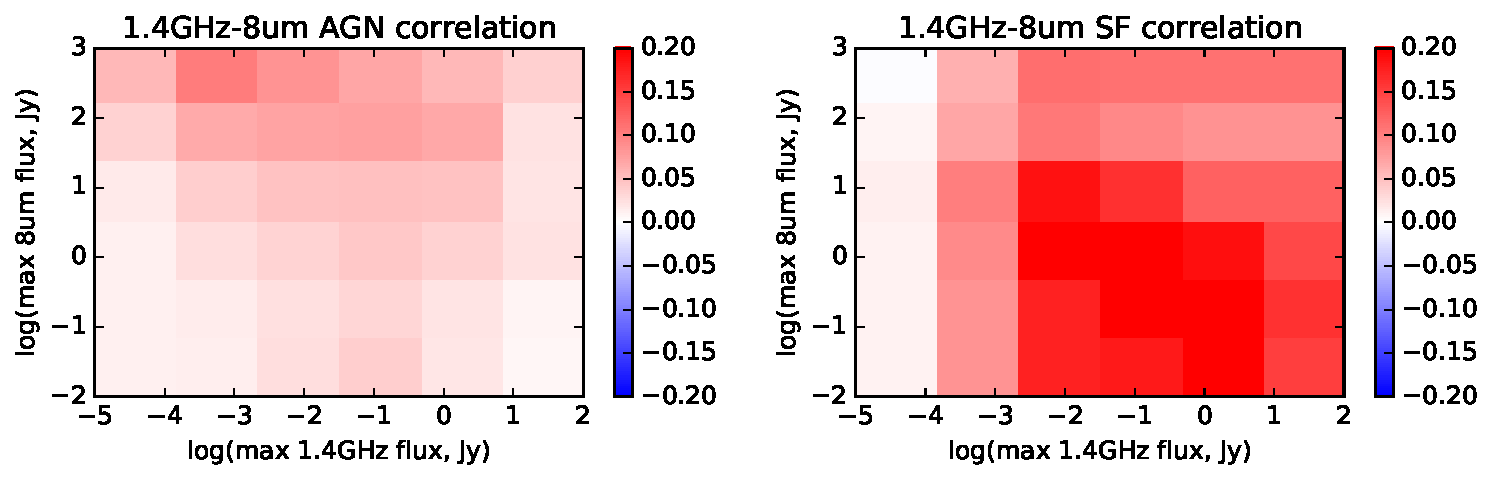
\includegraphics[width=6in]{images/sim_correlation_agn_and_sf.pdf}
\caption{5' pixels}
\label{fig:simagnlfcorrelations}
\end{figure}






\section{Residual foregrounds and cross power spectrum limits}

NEED TO START REWRITING THIS SECTION...to frame it as both a study of the unresolved broadband foreground residuals (ie, after point source masking/subtraction) and the first limits on the cosmological cross spectrum

% why the MWA?
In this section we perform a wide band power spectrum and foreground analysis on MWA observations. Details on the MWA instrument are given by \citet{tingay13}, but we summarize here some salient facts. The MWA is an ideal instrument for a 21\,cm--IR cross correlation experiment owing to its high surface brightness sensitivity and wide field of view, permitting analysis of many sky fourier modes in a short amount of time, necessary for averaging down foreground residuals in the cross spectrum. The array is comprised of 128 antenna tiles, each with $\sim20\,\text{m}^2$ collecting area over $150-200\,$MHz, spread quasi-randomly over a radius of 1.5\,km to achieve nearly complete $uv$ coverage in wide band images even without rotation synthesis. Each tile is a $4\times4$ phased array of dual-polarization bowtie dipoles summed by a delay-line beamformer, whose output beam is steerable in few degree increments across the sky. 

% observations
To assess both the level of systematics and noise in the MWA images and their ramifications for our cross correlation analysis, we perform our power spectrum analysis on observations of four different depths: 2\,min, 26\,min, 3\,hr, and 32\,hr. We use data from the MWA's high band study of its ``EOR0'' deep integration field, centered at $(\text{RA}, \text{Dec})=(0,-27^\circ)$. The two shallower observations are zenith pointed at hour angles centered on 00:00, while the two deeper observations synthesize pointed observations at the EOR0 field center observed from hour angles on either side of 00:00. For simplicity and because we are not sensitivity limited, we only use the EW instrumental polarization.

%wide band power spectrum processing (note related to k//=0 bin of the cube power spectrum, see Appendix)
Quality control, calibration, and processing into image cubes in described in detail by \citet{beardsley16}. In brief, the COTTER package \citep{AndreMWARFI}, based on AOFlagger\footnote{http://aoflagger.sourceforge.net} \citep{aoflagger} is used for initial identification and flagging of radio frequency interference, as well as time and frequency averaging to 2\,sec and 80\,kHz. Deeper quality cuts are performed using the delay transform \citep{parsons12b} to identify observations with subtle frequency structure due to wide band RFI or instrumental problems. A per-antenna, per-frequency calibration was performed to a sky model based the deep source catalogs of \citet{PattiCatalog1} and \citet{mwacs}, restricted such that only polynomial amplitudes and phases are allowed to vary between antennas. 

The calibration is a variant of StEFCal \citep{stefcal}, implemented as part of the Fast Holographic Deconvolution\footnote{https://github.com/EoRImaging/FHD} \citep{fhd} software used for imaging. FHD is run in ``first pass'' mode in which no deconvolution is performed, instead naturally weighted dirty images are produced from the measured and modeled visibilities, respectively, as well as a image of the point spread function (ie, fourier transform of the $uvf$ space sampling function). 

We apply uniform weighting by dividing by the absolute value of the fourier transform of the point spread function image, then form the inverse variance weighted power spectrum estimate as
\begin{equation}
	C(\ell)=\frac{\sum_{\vec{\ell}}|\tilde{I}_\text{uni}(\vec{\ell})w(\vec{\ell})|^2}{\sum_{\vec{\ell}}|w(\vec{\ell})|^2}
\end{equation}
where $w(\vec{\ell})=\text{FT}[I_\text{PSF}(\theta)](\vec{\ell})$. We estimate the thermal noise power spectrum by computing the power spectrum as above but using the odd minus even difference cube which contains only thermal noise.

SHOW THE UNIFORMLY WEIGHTED IMAGE AND THE SAMPLING

%take-aways
Figure XX shows XNTHOUNSTHESNTUHSNTOHUNETHUNTHEUNOT
	show both the 2 minute, and the 32 hour, and make the point that just as with IR, averaging is not necessary for noise, but for systematics



ATLAS image analysis



We compute the mean in source-free regions, and find a maximum airglow of roughly $5\times10^3$ kJy/sr across all the observations, of order 19 AB mag/arcsec$^2$. This value is consistent with the worst cases observed in the continuum airglow near $1\mu$m by \citet{sullivan12}.

Appendix \ref{sec:Pshot}

\section{Sensitivity study}




NEED TO START REJIGGERING THIS SECTION

We adapt the cross spectrum sensitivity results of \citet{lidz09} to our case of measuring the 21\,cm--IR cross spectrum of broadband images with noise and foreground residuals. 
\begin{equation}
\label{eqn:sense1}
	\sigma_{21,\IR}^2(\vec{\ell})=\frac{1}{2}[C^2_{21,\IR}(\vec{\ell})+\sigma_{21}(\vec{\ell})\sigma_{\IR}(\vec{\ell})]
\end{equation}
\begin{equation}
\label{eqn:sense2}
	\sigma_{21}^2(\vec{\ell})=[C_{21,\cosmo}(\vec{\ell})+C_{21,\fg}(\vec{\ell})+C_{21,\therm}(\vec{\ell})]^2
\end{equation}

\begin{equation}
\label{eqn:sense3}
	\sigma_{\IR}^2(\vec{\ell})=[C_{\IR,\cosmo}(\vec{\ell})+C_{\IR,\fg}(\vec{\ell})+C_{\IR,\shot}(\vec{\ell})]^2
\end{equation}
where $\cosmo$ signifies the cosmological component of the signal from the EOR, $\fg$ signifies residual foregrounds, $\therm$ signifies thermal noise in 21\,cm images, and $\shot$ signifies photon shot noise in IR images. 


Though these are the general forms of these equations, we omit the thermal and photon shot noise contributions in the rest of this section, as we have shown them to be negligible in Sections \ref{sec:pspec21fg} and \ref{sec:pspecIRfg}. We also omit the sample variance terms as they become important only in the SNR $\sim1$ regime. 

Now suppose we evaluate the 2D cross spectrum as in Eqn. \ref{eqn:Cldefcross}, and bin it in annuli such that bin $\ell$ contains containing $N_\ell$ $\ell$ cells. Then the noise decreases as
\begin{equation}
	\sigma_{21,\IR}^2(\ell) = \frac{\sigma_{21,\IR}^2(\vec{\ell}) }{N_\ell}
\end{equation}

Then substituting Eqns. \ref{eqn:sense1}-\ref{eqn:sense3} into the above equation and omitting factors of order unity, we find that the signal to noise ratio $\SNR(\ell)$ of the measurement of cross spectrum mode $\ell$ is given by
\begin{equation}
	\SNR(\ell) = \sqrt{
		2N_\ell
	\left(\frac{C_{21,\cosmo}(\vec{\ell})  }{ C_{21,\fg}(\vec{\ell}) }\right)
	\left(\frac{C_{\IR,\cosmo}(\vec{\ell})  }{ C_{\IR,\fg}(\vec{\ell}) }\right)
	}
\end{equation}

Let us optimize the SNR by using only two bins, $\ell_1=\ell_\text{max}/4$ and $\ell_2=3\ell_\text{max}/4$, where $\ell_\text{max}=\pi/d\theta$ and the cell size is given by $d\ell=2\ell_\text{max}/N=2\pi/\theta_\text{FOV}$. Now let's derive some intuition into $N_\ell$ by writing it as $N_\ell=(\ell_\text{max}/d\ell)^2F_\ell=(\theta_\text{FOV}/2d\theta)^2F_\ell$, where $F_\ell$ is an order unity quantity equal to the fraction of all $\vec{\ell}$ cells included in bin $\ell$.

%\begin{equation}
%	\SNR(\ell) = \frac{\theta_\text{FOV}}{2d\theta}  \sqrt{2F_\ell
%	\left(\frac{C_{21,\cosmo}(\vec{\ell})  }{ C_{21,\fg}(\vec{\ell}) }\right)
%	\left(\frac{C_{\IR,\cosmo}(\vec{\ell})  }{ C_{\IR,\fg}(\vec{\ell}) }\right)
%	}
%\end{equation}

\begin{eqnarray}
	\SNR(\ell)&=&XX \left(\frac{\theta_\text{FOV}}{20^\circ}\right)\left(\frac{5'}{d\theta}\right)\left(\frac{F_\ell}{1}\right)^{1/2}\left(\frac{\alpha_{21}}{0.1}\right)^{1/2}
\end{eqnarray}
where the fraction of 21\,cm foregrounds remaining after subtraction is given by $\alpha_{21}\equiv C_{21,\res}/C_{21,\fg}$, and the fraction of IR foregrounds removed by masking is assumed to be XXX. REMEMBER, WE CAN'T MASK OUR WAY TO THE SIGNAL BECAUSE OF THE INTRAHALO
-LIGHT






\section{Discussion}

\appendix

\section{Power spectrum of photon shot noise}
\label{sec:Pshot}

In Sec. \ref{sec:pspecIRfg} we measure the maximum airglow to be $I_\text{air}=5\times10^3$ kJy/sr, and in this appendix we calculate the power spectrum of this photon shot noise. We must observe that the mean number of photons collected by a pixel during each observation is $\langle N_\text{ph}\rangle=I_\text{air}At_\text{int} \Delta f d\theta^2/hf$, where $A=(0.5\,\text{m})^2$ is the collecting area of ATLAS, $t_\text{int}=30\,$sec, $\Delta f$ and $f$ are the frequency bandwidth and center frequency of I band, and $d\theta$ is the pixel size. The passband has $\Delta\lambda=150\,$nm and $\lambda=800\,$nm. 

The shot noise contribution to the power spectrum is given by
\begin{equation}
C_{\IR, \shot}(\vec{\ell}) = \left\langle\left|\sum_{m,n}I_\shot(m,n)e^{-2\pi i(ma+nb)/N}\right|^2\right\rangle \frac{d\theta^2}{N^2}
\end{equation}
where $I_\shot(m,n)\equiv I(m,n)-\langle I(m,n)\rangle$ denotes the photon shot noise contribution to pixel (m,n), and $N$ is the number of pixels on each side of the square image. Then using the fact that the shot noise is uncorrelated between different pixels, we find
\begin{equation}
C_{\IR, \shot}(\vec{\ell}) = \sum_{m,n}\langle I^2_\shot(m,n)\rangle \frac{d\theta^2}{N^2}
\end{equation}
Note that $I(m,n)=N_\text{ph}(m,n)hf/\Delta f A t_\text{int}d\theta^2$ and $\langle N_\text{ph}^2\rangle = \langle N_\text{ph}\rangle$, so we have
\begin{equation}
C_{\IR, \shot}(\vec{\ell}) = \langle N_\text{ph}\rangle \left(\frac{hf}{\Delta f A t_\text{int}d\theta^2}\right)^2 d\theta^2
\end{equation}

\begin{equation}
C_{\IR, \shot}(\vec{\ell}) =\frac{I_\text{air}h\lambda}{\Delta \lambda A t_\text{int}}
\end{equation}

NOTE THAT $C_\shot$ DECREASES WITH BINNING IN THE CROSS SPECTRUM, BUT NOT IN THE AUTO SPECTRUM!!!!!!!!!!!!!!!!!!!!!!!

\section{Relation between the power spectrum of image cubes and broadband images}
\label{sec:pspecrelation}

NOTE THAT THIS ONLY HOLDS FOR LARGE ELL OVER A SMALL FIELD OF VIEW

We focus in this paper on the spherical power spectrum of broadband images, $C_\ell$,  instead of that of image cubes, $P(\vec{k})$, as 21\,cm observations have focused on. Here we work out the relation between the two to facilitate comparison with past 21\,cm power spectrum results. In particular, we calculate the scaling factor $B$ relating the purely transverse modes of the power spectrum $P(k_\perp,k_\parallel=0)$ of a image cube $I(\theta_x,\theta_y,f)$ to the spherical power spectrum of a broad band image $C_\ell$ as
\begin{equation}
P(k_\perp,k_\parallel=0) = B C_{\ell(k_\perp)}
\end{equation}

Using the fourier transform convention discussed in Sec. \ref{sec:pspecconventions}, the left side of the equation is given by
\begin{equation}
P(k_\perp,k_\parallel=0) = \frac{1}{N_\perp^2 N_\parallel dV}\langle|\tilde{I}(k_x,k_y,k_\parallel=0)|^2\rangle
\end{equation}
where $N_\perp\equiv N_x=N_y$ is the number of pixels in each of the two transverse dimensions of the image cube, and $N_\parallel$ is the number of pixels in the line of sight (ie, frequency) dimension. The comoving pixel volume is $dV = (D_c d\theta)^2 (\Delta D_c/N_\parallel)$, where $D_c$ is the line of sight comoving distance from the present day to the center of the cube, and $\Delta D_c$ is the comoving line of sight thickness of the cube. Lastly, recall that $k_\perp$ is related to $k_x$ and $k_y$ as $k_\perp=\sqrt{k_x^2+k_y^2}$.

Now substituting the definition of the fourier transform, we find

\begin{equation}
P(k_\perp,k_\parallel=0) =\frac{1}{N_\perp^2 N_\parallel dV}\left\langle\left|dV\sum_{\theta_x,\theta_y,f}I(\theta_x,\theta_y,f)e^{iD_c(k_x\theta_x+k_y\theta_y)}\right|^2\right\rangle
\end{equation}

Simplifying and writing this in terms of the broadband image $I_{\Delta f}(\theta_x,\theta_y)\equiv\frac{1}{N_\parallel}\sum_f  I(\theta_x,\theta_y,f)$, we find

\begin{equation}
P(k_\perp,k_\parallel=0) =(D_c^2 \Delta D_c)
\frac{d\theta^2}{N_\perp^2}\left\langle\left|\sum_{\theta_x,\theta_y}I_{\Delta f}(\theta_x,\theta_y)e^{iD_c(k_x\theta_x+k_y\theta_y)}\right|^2\right\rangle
\end{equation}

Now denote $k_x=a\cdot dk$, $k_y=b\cdot dk$, $\theta_x=m\cdot d\theta$, and $\theta_y=n\cdot d\theta$, where $dk = 1/N_\perp D_c d\theta$. 

\begin{equation}
P(k_\perp(\ell(a,b)),k_\parallel=0) =(D_c^2 \Delta D_c)
\frac{d\theta^2}{N_\perp^2}\left\langle\left|\sum_{m,n}I_{\Delta f}(m,n)e^{2\pi i(am + bn)/N_\perp}\right|^2\right\rangle
\end{equation}

Comparing with Equations \ref{eqn:Cldef}, \ref{eqn:elldef}, and \ref{eqn:elldef2}, we see that $B\equiv P(k_\perp,k_\parallel=0)/ C_{\ell(k_\perp)}=D_c^2 \Delta D_c$ and $\ell=D_c k_\perp$.

%% The reference list follows the main body and any appendices.
%% Use LaTeX's thebibliography environment to mark up your reference list.
%% Note \begin{thebibliography} is followed by an empty set of
%% curly braces.  If you forget this, LaTeX will generate the error
%% "Perhaps a missing \item?".
%%
%% thebibliography produces citations in the text using \bibitem-\cite
%% cross-referencing. Each reference is preceded by a
%% \bibitem command that defines in curly braces the KEY that corresponds
%% to the KEY in the \cite commands (see the first section above).
%% Make sure that you provide a unique KEY for every \bibitem or else the
%% paper will not LaTeX. The square brackets should contain
%% the citation text that LaTeX will insert in
%% place of the \cite commands.

%% We have used macros to produce journal name abbreviations.
%% AASTeX provides a number of these for the more frequently-cited journals.
%% See the Author Guide for a list of them.

%% Note that the style of the \bibitem labels (in []) is slightly
%% different from previous examples.  The natbib system solves a host
%% of citation expression problems, but it is necessary to clearly
%% delimit the year from the author name used in the citation.
%% See the natbib documentation for more details and options.

%\bibliography{xcor_paper}
\bibliography{xcor_paper_new}


\end{document}
